
%---------------------------------------------------------------------
%---------------------------------------------------------------------
%----  CHAPTER 2, Background Research on Rare Event Simulation -------
%---------------------------------------------------------------------
%---------------------------------------------------------------------
\chapter{Background Research on Rare-Event Simulation}  
\label{ch:Background Research on Rare Event Simulation}
In this chapter background research on rare-event simulation is reviewed, including the models and the simulation algorithms. First, a descriptive presentation of the different models is conducted, where both Markovian and non-Markovian examples are given...

\section{Models, Markovian and Non-Markovian}
\label{sec:Models, Markovian and Non-Markovian}
In the current work different types of models are considered, where one of the main classifications is the requirement of memory or not. As introduced, a model without memory requirement is considered Markovian, and by opposition one that requires memory is non-Markovian. A Markovian model is a stochastic model that changes based on a random factor, and the future state depends only on the current one, not on previous states or events leading to it. A non-Markovian model does not fulfill this property, therefore only knowing the current state is not enough to completely describe the current situation. In a non-Markovian model the followed path of states and the events that lead to them are relevant as well.

\subsection{Markov Chain}
\label{sub:Markov Chain}
A Markov chain model is a static Markovian model, composed of states and transitions, where each state has incoming and outgoing transitions. Each of the outgoing transitions has a probability of being followed, and by definition, this probability only depends on the current state, not on previous visited states. Therefore, if a simulation is run over a Markov chain and at two different points in time the same state is reached, there is no difference between the execution status at those points, and all the following possible paths have the same probability in both scenarios. A simple Markov chain with three states and their transitions is presented in Figure~\ref{fig:Simple Markov Chain Model}. The values shown over the transitions correspond to their rates, and the probability is calculated with this value over the sum of all outgoing transitions of the state.

\begin{figure}[t]
\center
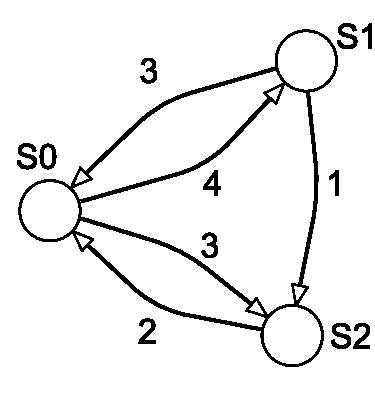
\includegraphics[width=.25\textwidth]{Model_Markov_Chain_Simple.pdf}
\caption{Simple Markov Chain Model}
\label{fig:Simple Markov Chain Model}
\end{figure}

The distribution of the time remaining in a state is memoryless, which is modeled with an exponential distribution: $f(x) = \lambda e^{-\lambda x}$, $F(x) = 1 - e^{-\lambda x} \ (x \geq 0)$ \cite{haas:spn}. The average firing time for a transition with rate $\lambda$ is $\lambda^{-1}$. Moreover, in a state with $t$ outgoing transitions the average time spent is:
$$ Average\ Time = \displaystyle\frac{\displaystyle 1}{\displaystyle\sum\limits_{i=0}^t (rate_i)} $$


In the example presented in Figure~\ref{fig:Simple Markov Chain Model} the transition matrix is:

\[ Q = \left( \begin{array}{ccc}
-7 & 4 & 3 \\
3 & -4 & 1 \\
2 & 0 & -2 \end{array} \right)\]


\section{Monte Carlo Simulation Algorithm} 
A Monte Carlo simulation algorithm follows a standard Monte Carlo method \cite{montecalro}. Whenever a decision needs to be made, a random result is generated based on the probability of each of the possible choices. Considering a Markov chain as the underlying model for a simulation executing a Monte Carlo algorithm, given the current state there are some outgoing transitions, each of them with a probability of being executed next...


\newpage

\begin{lstlisting}[caption={\texttt{Abstract Representation} -  Monte Carlo Algorithm}, label=code:monte_carlo_code, showlines=true]
// Initialization, set current state to the initial state
state *current_state = initial_state;

// Main simulation loop
while ( ! stop_condition_reached() )
{
  int tran, selected_tran;	
  // Array with all the outgoing transitions rates from the current state
  double trans_rates[] = get_out_transitions_rates( current_state );
  int trans_count = get_out_transitions_count( current_state );

  // Calculate the sum of all the outgoing transitions rates
  double total_rates = 0;	
  for( tran = 0; tran < trans_count;  tran++)
    total_rates += trans_rates[ tran ];		

  // Calculate the average time spent in the state
  double time_spent = 1.0 / total_rates;
  // Evaluate measures defined over the current state
  evaluate_measures( current_state, time_spent );

  // Randomly select one outgoing transitions, based on their rates
  double random_value = generate_random_value( 0, total_rates );
  for( tran = 0; tran < trans_count;  tran++)
  {
    if ( random_value <  trans_rates[ tran ] ) 
    {
      selected_tran = tran;
      break;
    }
    random_value -= trans_rates[ tran ];
  }	
		
  // Execute the selected transition, and update the current state
  current_state = fire_transition( current_state, selected_tran );
}

\end{lstlisting}

